% Shared preamble + layout macros for Ratio competitive component specs.
% Each <slug>.tex \input{}s this, then opens \begin{document}. Compiled
% per-component to its own PDF by rules_tectonic (see spec.bzl / BUILD).
\documentclass[11pt,letterpaper]{article}
\usepackage[T1]{fontenc}
\usepackage[utf8]{inputenc}
\usepackage{lmodern}
\usepackage{microtype}
\usepackage[margin=0.9in]{geometry}
\usepackage{xcolor}
\usepackage{graphicx}
\usepackage{booktabs}
\usepackage{array}
\usepackage{colortbl}
\usepackage{pifont}
\usepackage{enumitem}
\usepackage[most]{tcolorbox}
\usepackage{hyperref}

% ── Brand palette (shared with the Ratio papers) ────────────────────
\definecolor{ratioInk}{HTML}{0F2418}
\definecolor{ratioAccent}{HTML}{1B6440}
\definecolor{ratioMid}{HTML}{679177}
\definecolor{ratioRule}{HTML}{C3D6BF}
\definecolor{ratioTint}{HTML}{E6EFE2}
\definecolor{posGreen}{HTML}{1F6B45}
\definecolor{negGray}{HTML}{666666}

\hypersetup{colorlinks=true, linkcolor=ratioAccent, citecolor=ratioAccent, urlcolor=ratioAccent}
\setlist[itemize]{leftmargin=1.3em, itemsep=2.5pt, topsep=2pt}
\pagestyle{plain}
\setlength{\parindent}{0pt}
\setlength{\parskip}{4pt}

\newcommand{\yes}{{\color{posGreen}\ding{51}}}
\newcommand{\no}{{\color{negGray}\ding{55}}}

% ── Header banner: \spechead{Title}{slug} ───────────────────────────
\newcommand{\spechead}[2]{%
  \noindent\begin{tcolorbox}[colback=ratioInk, colframe=ratioInk, arc=4pt,
      left=14pt, right=14pt, top=11pt, bottom=11pt, boxrule=0pt]
    {\sffamily\footnotesize\color{ratioRule}
      RATIO COMPONENT SPEC \;\textbullet\; benchmarked to the wealth-tech stack
      \;\textbullet\; \texttt{#2}}\\[3pt]
    {\sffamily\bfseries\LARGE\color{white} #1}
  \end{tcolorbox}\par\vspace{8pt}}

% ── Section heading: \specsection{Name} ─────────────────────────────
\newcommand{\specsection}[1]{%
  \vspace{6pt}{\sffamily\large\bfseries\color{ratioAccent} #1}\par
  \vspace{1pt}{\color{ratioRule}\rule{\linewidth}{1pt}}\par\vspace{3pt}}

% ── Highlighted "Ratio mapping" box ─────────────────────────────────
\newtcolorbox{ratiobox}{colback=ratioTint, colframe=ratioMid, boxrule=0.8pt,
  arc=3pt, left=9pt, right=9pt, top=7pt, bottom=7pt}

% ── Status footer box ───────────────────────────────────────────────
\newtcolorbox{statusbox}{colback=ratioRule!35, colframe=ratioRule, boxrule=0.6pt,
  arc=2pt, left=8pt, right=8pt, top=5pt, bottom=5pt}

% ── "Advertised by" two-column table helper ─────────────────────────
\newcommand{\advrow}[2]{\textbf{#1} & #2 \\}

\newcommand{\pmark}{{\color{ratioTan}\textbf{\textasciitilde}}}
\begin{document}

\begin{center}
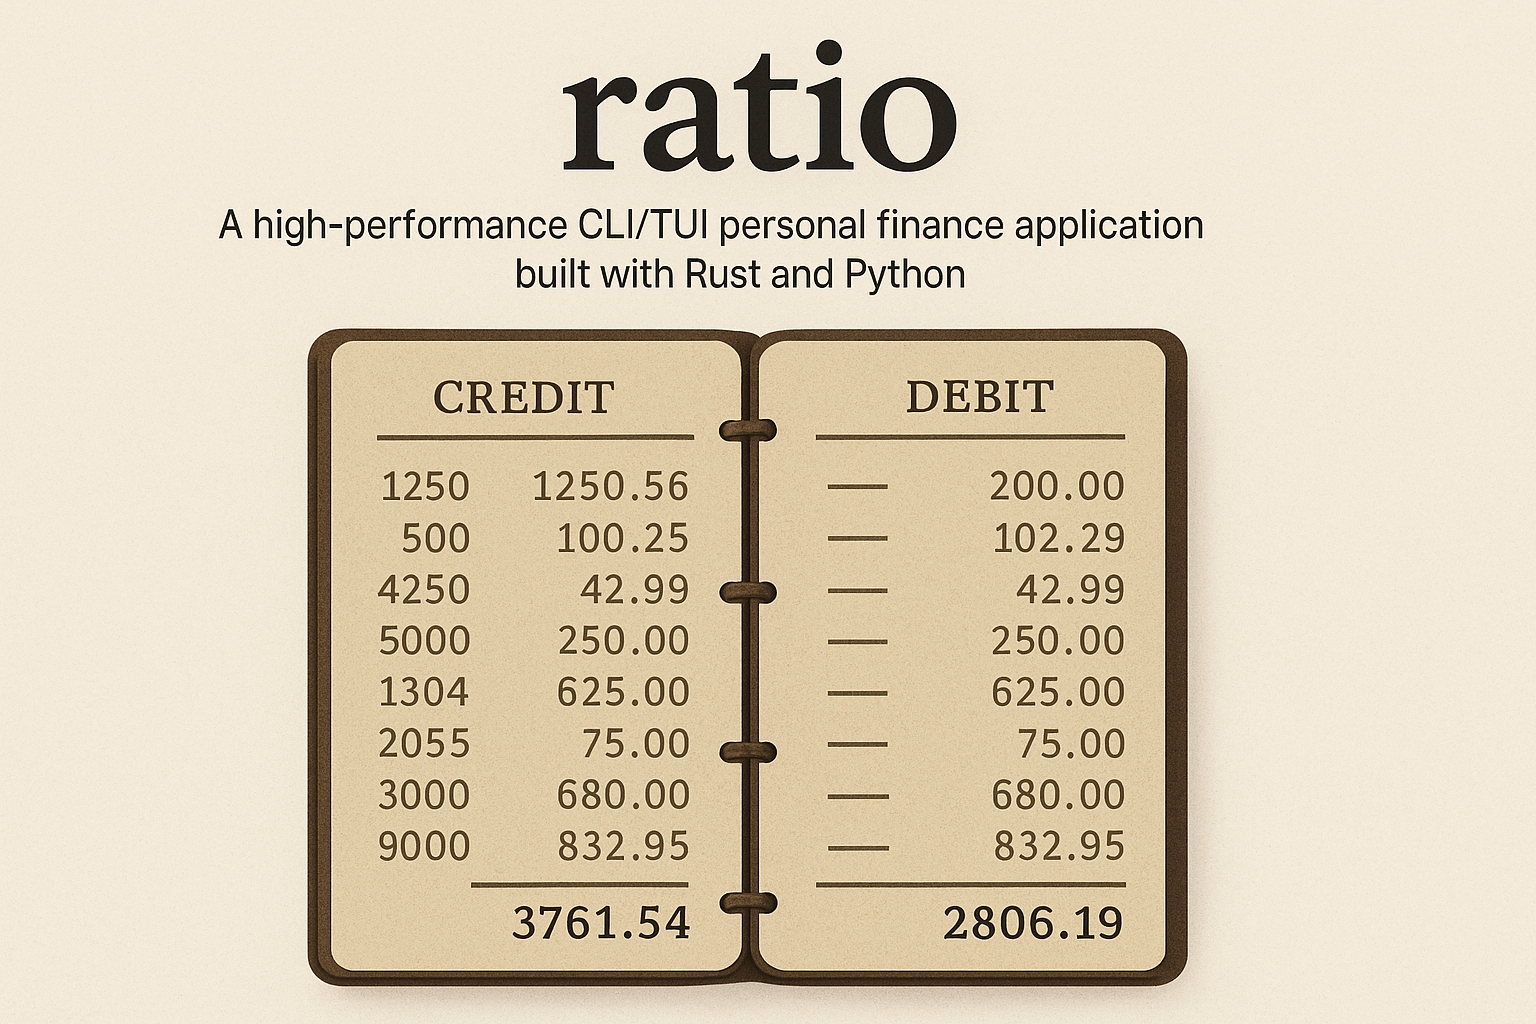
\includegraphics[width=0.26\textwidth]{../../images/ratio.png}\\[6pt]
{\sffamily\bfseries\LARGE\color{ratioInk} Wealth-Tech Component Architecture}\\[2pt]
{\sffamily\large\color{ratioBrown} Competitive scaffold --- one Ratio spec per advertised component}
\end{center}
\vspace{4pt}

This catalog was scaffolded from a June 2026 scrape of the published
component/feature architecture of SS\&C Black Diamond (primary anchor), Orion,
Addepar, and Envestnet Tamarac. Each row links to a standalone component spec
(\texttt{<slug>.pdf}); each spec records the advertised capabilities, the
benchmark sources, and how the component maps onto Ratio's proven-kernel
architecture. \yes\ advertised \quad \pmark\ partial / adjacent \quad \no\ not advertised.

\vspace{6pt}
{\renewcommand{\arraystretch}{1.3}\setlength{\tabcolsep}{4pt}\sffamily\footnotesize
\begin{tabular}{@{}p{0.30\linewidth}*{4}{>{\centering\arraybackslash}p{0.052\linewidth}}p{0.30\linewidth}@{}}
\rowcolor{ratioInk}
\textbf{\color{white}Component (slug)} & \textbf{\color{white}BD} & \textbf{\color{white}Ori} & \textbf{\color{white}Add} & \textbf{\color{white}Tam} & \textbf{\color{white}Ratio placement} \\
\arrayrulecolor{ratioSand}\midrule
Portfolio Accounting \& Reporting \newline {\scriptsize\texttt{portfolio-accounting}} & \yes & \yes & \yes & \yes & Trusted core (proven) \\
\rowcolor{ratioCream}
Data Aggregation \& Reconciliation \newline {\scriptsize\texttt{data-aggregation}} & \yes & \yes & \yes & \pmark & Fact plane (provenance) \\
Trading \& Rebalancing \newline {\scriptsize\texttt{trading-rebalancing}} & \yes & \yes & \yes & \yes & Control plane $\to$ core \\
\rowcolor{ratioCream}
Models, Managed Accts \& Marketplace \newline {\scriptsize\texttt{model-management}} & \yes & \yes & \pmark & \yes & Control plane \\
Proposal Generation \newline {\scriptsize\texttt{proposal-generation}} & \yes & \pmark & \pmark & \yes & Sim over core \\
\rowcolor{ratioCream}
Billing \& Revenue Management \newline {\scriptsize\texttt{billing}} & \yes & \yes & \pmark & \yes & Control plane $\to$ core \\
Client Experience Portal \newline {\scriptsize\texttt{client-portal}} & \yes & \yes & \yes & \yes & Presentation tier \\
\rowcolor{ratioCream}
CRM \newline {\scriptsize\texttt{crm}} & \yes & \yes & \pmark & \yes & Extension tier \\
Compliance \& Surveillance \newline {\scriptsize\texttt{compliance}} & \yes & \yes & \pmark & \yes & Control plane + record \\
\rowcolor{ratioCream}
Risk Analytics \& Scenario Modeling \newline {\scriptsize\texttt{risk-analytics}} & \pmark & \yes & \yes & \pmark & Analytical + sim \\
Practice Analytics \& BI \newline {\scriptsize\texttt{business-intelligence}} & \yes & \yes & \pmark & \pmark & Analytical tier \\
\rowcolor{ratioCream}
Alternative Investments Servicing \newline {\scriptsize\texttt{alternative-investments}} & \yes & \pmark & \yes & \pmark & Core (dimensions) \\
Integrations, API \& Marketplace \newline {\scriptsize\texttt{integrations}} & \yes & \yes & \yes & \yes & API + extension \\
\rowcolor{ratioCream}
AI \& Natural-Language Insights \newline {\scriptsize\texttt{ai-insights}} & \pmark & \yes & \yes & \pmark & Authoring (fenced) \\
Access Control \& Data Governance \newline {\scriptsize\texttt{data-governance}} & \pmark & \pmark & \yes & \pmark & API boundary \\
\rowcolor{ratioCream}
Trust / Retirement / Insurance \newline {\scriptsize\texttt{specialized-servicing}} & \yes & \pmark & \pmark & \no & Control plane + core \\
\arrayrulecolor{ratioSand}\bottomrule
\end{tabular}}

\vspace{8pt}
\begin{ratiobox}
\textbf{Reading the ``Ratio placement'' column.} It records where each component
sits relative to the machine-checked kernel. Only \emph{portfolio accounting} and
the conserved-dimension parts of \emph{alts} / \emph{specialized servicing} live
in the trusted core; everything else is control plane, fact plane, analytics,
presentation, or fenced AI authoring --- expressive surfaces that, by
construction, cannot violate conservation. This is the structural reason Ratio can
match the incumbents' breadth without enlarging the surface on which a correctness
bug can exist.
\end{ratiobox}

\begin{statusbox}
\footnotesize
\textbf{Status / disclaimer:} scaffold generated from public marketing pages
(June 2026); coverage marks reflect Ratio's reading of those pages, not a feature
audit, and capabilities evolve. Black Diamond is a trademark of SS\&C
Technologies; Orion, Addepar, and Tamarac are trademarks of their respective
owners. Ratio is independent and unaffiliated. Build all specs with
\texttt{bazel build //competitive/specs:all\_specs}.
\end{statusbox}
\end{document}
